\chapter{GitHub Enterprise and GitHub Cloud}

\section{About GitHub}

The GitHub integration supports self-hosted GitHub Enterprise or GitHub Cloud.  The integration configurations
are virtually the same for each GitHub platform.  Minor differences may exist due to license or subscription
limitations of your GitHub platform type.  

The GitHub integration, as with other SCM integrations, uses web hooks to emit events to the \cxoneflow endpoint.
GitHub has both organization-level and repository-level webhook configurations
that can be used for simple integration scenarios.  \cxoneflow can also be configured as a GitHub Application
for easier deployment and visibility of deployment.

Deployment as a GitHub Application is the recommended deployment method.  It offers a single location where
\cxoneflow can be integrated into all organizations in a GitHub Enterprise instance or GitHub Cloud subscription.
When the GitHub application is defined by a logged in user, the scope of deployment may be limited by the access rights
the user has to each organization.  The \cxoneflow GitHub application runs with limited rights in each installed
organization, but it may require a user with administrative access across all organizations for deployment.


\section{GitHub Application Configuration}

\subsection{Configuring the Application Definition}

The GitHub Application definition determines the owner of the application.  The definition can
be created with an organization as owner or a user as owner.  The configuration method is the same
for each type of ownership.  Deploying with a user as application owner may be disruptive if the user
account is deleted or suspended.

\noindent\\Once the type of ownership is decided, the GitHub Application configuration page can be found in the following
locations:

\begin{itemize}
    \item \textbf{Organization Ownership:} Organization->Settings>Developer Settings->GitHub Apps
    \item \textbf{User Ownership:} User Icon (Top Right)->Settings->Developer Settings->GitHub Apps
\end{itemize}

\noindent\\The following steps can be followed to configure the \cxoneflow GitHub App:

\begin{enumerate}
    \item To start the configuration, click the button "New GitHub App". Figure \ref{fig:gh-new-app} shows
    the GitHub App page with the button to start the configuration in GitHub Enterprise.
    \item Provide a name for the GitHub App as depicted in Figure \ref{fig:gh-app-cfg-1}.  Any name
    can be used, but \cxoneflow is suggested.
    \item Optionally provide a description that is displayed to the users.
    \item Provide a URL that can be used to find information about the \cxoneflow GitHub App.  Any URL
    can be used; the URL to the \cxoneflow GitHub page \textbf{https://github.com/checkmarx-ts/cxone-flow}
    is suggested.
    \item Scroll to the \textbf{Webhook} configuration section; the settings prior to the web hook configuration
    are optional and not used by \cxoneflow.
    \item Provide the URL to the \cxoneflow endpoint with the \textbf{/gh} suffix as shown in Figure \ref{fig:gh-app-cfg-2}.
    \item Provide the web hook secret value that is configured in the \cxoneflow YAML as described in Section \ref{sec:connection-element}.
    \item Scroll the the \textbf{Permissions} section and expand the \textbf{Repository Permissions} as shown in
    Figure \ref{fig:gh-app-cfg-3}.  The following permissions are required:
    \begin{itemize}
        \item Contents: Read-only
        \item Pull requests: Read and write
    \end{itemize}
    \item Scroll to the \textbf{Subscribe to events} section as shown in Figure \ref{fig:gh-app-cfg-4}.  The following events are required:
    \begin{itemize}
        \item Pull request
        \item Pull request review
        \item Push
    \end{itemize}
    \item Scroll to the \textbf{Where can this GitHub App be installed?} section and select \textbf{Any account} as shown in
    Figure \ref{fig:gh-app-cfg-5}.
    \item Click the \textbf{Create GitHub App} button.
    \item After the application is created, open the application settings \textbf{General} tab and scroll to the
    \textbf{Private keys} section as shown in Figure \ref{fig:gh-app-cfg-6}.
    \item Click the \textbf{Generate a private key} button.  A private key entry will appear and a file download will start.
    The contents of the download file is the PEM encoded private key that is to be stored as a secret.  See Section
    \ref{sec:api-auth-element} for configuration instructions to reference this GitHub App private key.
\end{enumerate}

\begin{figure}[ht]
    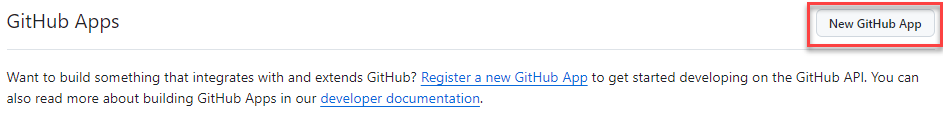
\includegraphics[width=\textwidth]{graphics/gh-new-app.png}
    \caption{New GitHub App Button}
    \label{fig:gh-new-app}
\end{figure}


\begin{figure}[ht]
    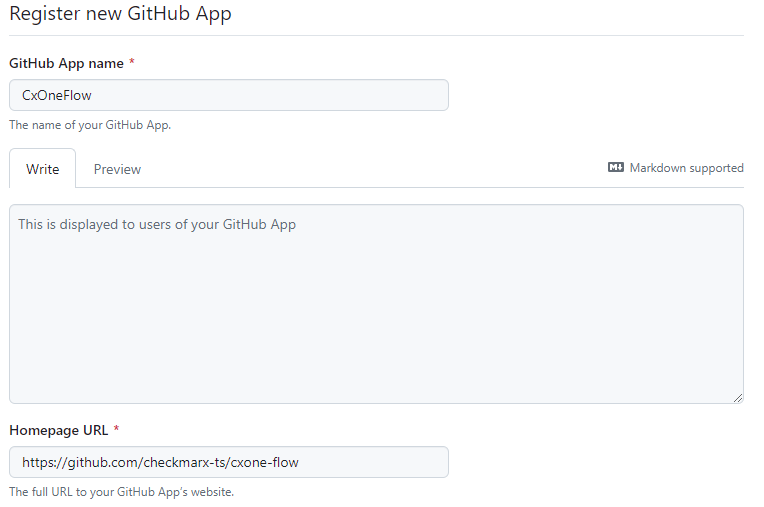
\includegraphics[width=\textwidth]{graphics/gh-app-cfg-1.png}
    \caption{GitHub App Name and URL Configuration}
    \label{fig:gh-app-cfg-1}
\end{figure}

\begin{figure}[ht]
    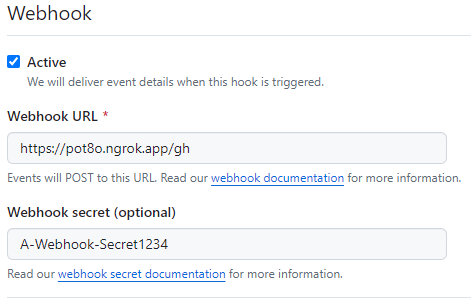
\includegraphics[width=\textwidth]{graphics/gh-app-cfg-2.png}
    \caption{GitHub App Webhook Configuration}
    \label{fig:gh-app-cfg-2}
\end{figure}

\begin{figure}[ht]
    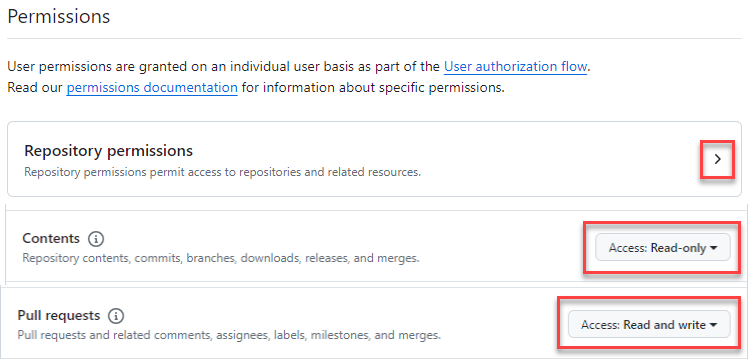
\includegraphics[width=\textwidth]{graphics/gh-app-cfg-3.png}
    \caption{GitHub App Permissions}
    \label{fig:gh-app-cfg-3}
\end{figure}

\begin{figure}[ht]
    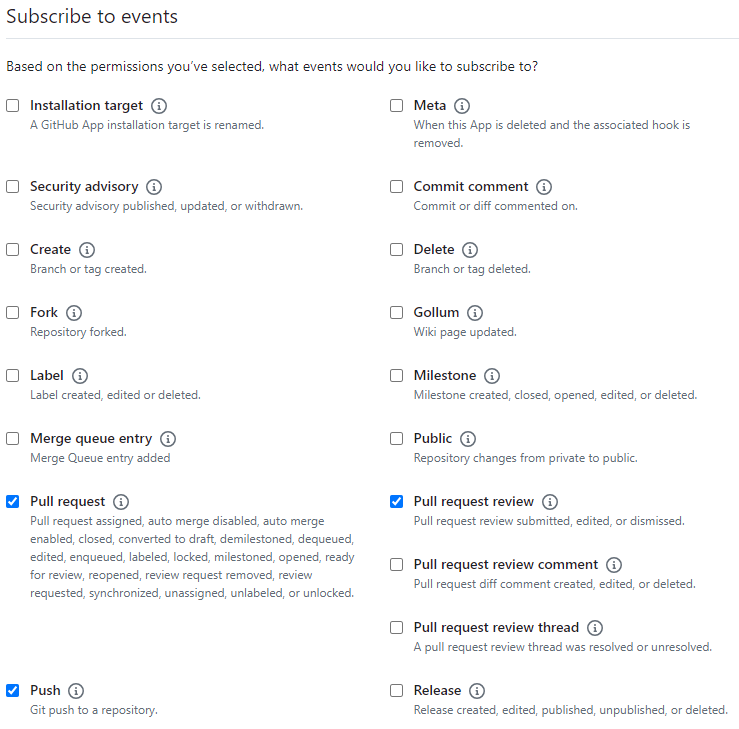
\includegraphics[width=\textwidth]{graphics/gh-app-cfg-4.png}
    \caption{GitHub App Event Subscriptions}
    \label{fig:gh-app-cfg-4}
\end{figure}

\begin{figure}[ht]
    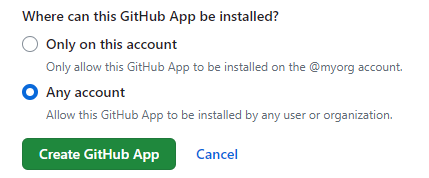
\includegraphics[width=\textwidth]{graphics/gh-app-cfg-5.png}
    \caption{GitHub App Install Scope}
    \label{fig:gh-app-cfg-5}
\end{figure}

\begin{figure}[ht]
    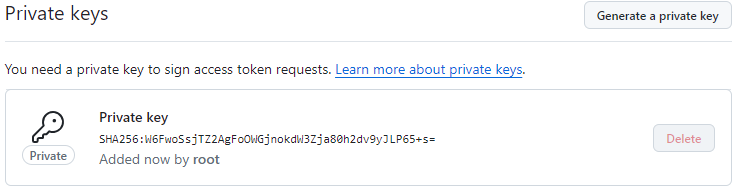
\includegraphics[width=\textwidth]{graphics/gh-app-cfg-6.png}
    \caption{GitHub App Private Keys}
    \label{fig:gh-app-cfg-6}
\end{figure}

\FloatBarrier

\subsection{Deploying the Application}

\textbf{Before deploying the application, it is recommended to configure the \cxoneflow YAML
so the endpoint will recognize events sent by the application.  See Section \ref{sec:gh-yaml-config} for guidance on the \cxoneflow
GitHub configuration.}

\noindent\\After the application is defined, deployment is performed from the application
definition page. The following steps can be followed to deploy the \cxoneflow GitHub App:

\begin{enumerate}
    \item Navigate to the GitHub App definition page and click the \textbf{Edit} button for the \cxoneflow
    application definition.  An example of this view is shown in Figure \ref{fig:gh-app-deploy-1}.
    \item Select the \textbf{Install App} tab on the left side of the view.  Figure \ref{fig:gh-app-deploy-2}
    shows the install view.\footnote{If the view shows only the organization that owns the \cxoneflow GitHub App definition,
    then the application visibility is configured to be private.  The application must be public to install in other organizations.}
    \item Click the \textbf{Install} button next to the organization where the application should be installed.
    \item An installation confirmation similar to that shown in Figure \ref{fig:gh-app-deploy-3} will be displayed.
    Click the \textbf{Install} button to complete installation.
    \item Repeat these steps to install the \cxoneflow GitHub App in all desired organizations.  Figure \ref{fig:gh-app-deploy-4}
    shows the view where the GitHub App has been installed in multiple organizations.
\end{enumerate}

\begin{figure}[ht]
    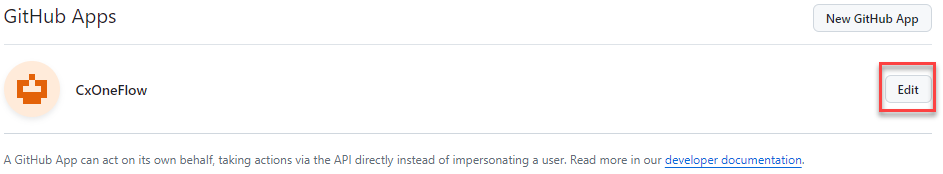
\includegraphics[width=\textwidth]{graphics/gh-app-deploy-1.png}
    \caption{GitHub App List}
    \label{fig:gh-app-deploy-1}
\end{figure}

\begin{figure}[ht]
    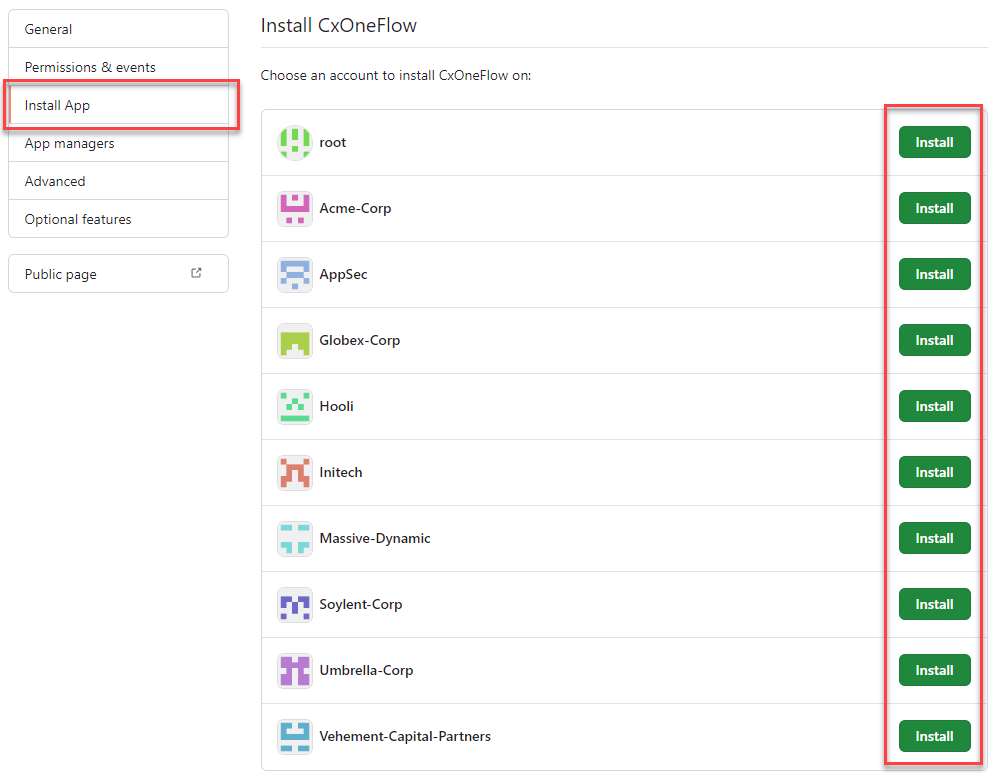
\includegraphics[width=\textwidth]{graphics/gh-app-deploy-2.png}
    \caption{GitHub App Install View}
    \label{fig:gh-app-deploy-2}
\end{figure}

\begin{figure}[ht]
    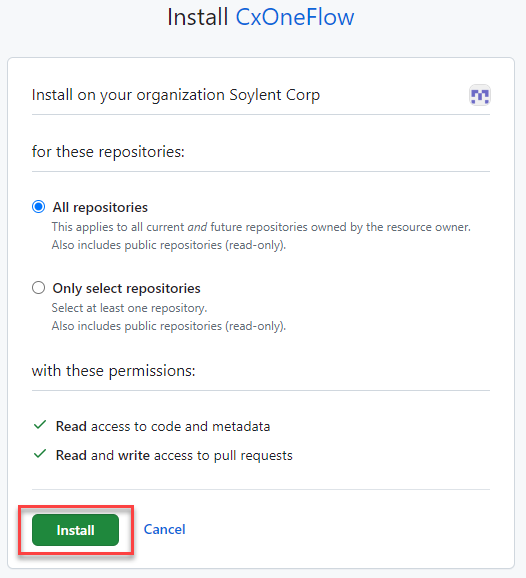
\includegraphics[width=\textwidth]{graphics/gh-app-deploy-3.png}
    \caption{GitHub App Install Confirmation}
    \label{fig:gh-app-deploy-3}
\end{figure}

\begin{figure}[ht]
    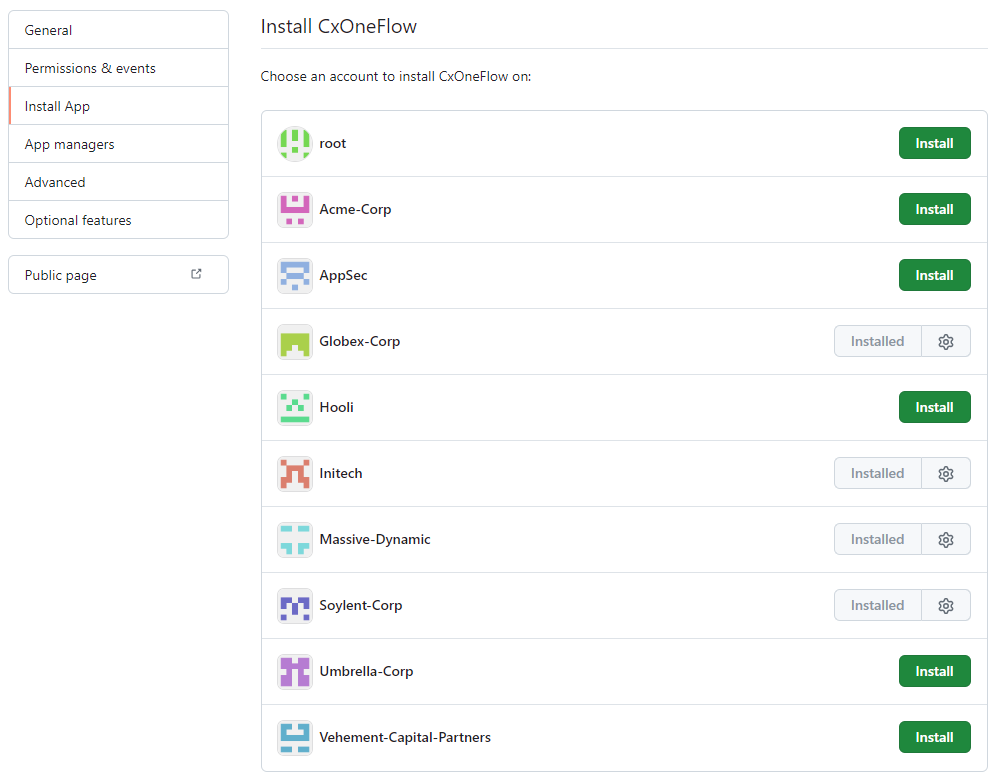
\includegraphics[width=\textwidth]{graphics/gh-app-deploy-4.png}
    \caption{GitHub App Installed Organization View}
    \label{fig:gh-app-deploy-4}
\end{figure}

\FloatBarrier

\subsection{GitHub App Management Recommendations}

\subsubsection{Repository Scope}

It is recommended that the application is installed for all repositories in an organization.  While it is possible to limit the
application to specific repositories, modifications to change the selected repositories may be difficult to manage.  Limiting
the repository scope may be useful for testing purposes but impractical for normal operations.

\subsubsection{Organization User App Management Permissions}

In each organization, a number of users may have the rights to manage applications that are installed on that organization.  It is
recommended to restrict the ability of organization users to manage installed applications.  Each organization user that can manage
GitHub Apps in that organization can suspend or remove the \cxoneflow application installation.

If the \cxoneflow application is deleted, this will be reflected in the \textbf{Install App} view as shown in Figure \ref{fig:gh-app-deploy-4}.
This is easy to periodically audit and discover when the application has been removed from an organization unintentionally or otherwise.
If the application is simply suspended, the \textbf{Install App} view will indicate the application is installed but will not indicate
that operation has been suspended.

The \cxoneflow logs do emit log entries when the GitHub App is suspended or removed. The listing below shows example log events
emitted when a user has modified the GitHub App on an organization.  If desired, monitoring for these log events may provide
an automated method of auditing when the GitHub App is no longer active for an organization.

\begin{code}{GitHub App Example Events}{}{}
[2024-10-03T13:10:30+0000][3219][GithubOrchestrator][INFO] Install event 'suspend': Initiated by [root] on Organization [Initech]
[2024-10-03T13:11:02+0000][3219][GithubOrchestrator][INFO] Install event 'deleted': Initiated by [root] on Organization [Initech]
\end{code}

\section{Webhook Configuration}

If it is not possible to use the GitHub App for \cxoneflow integration, webhook definitions can be configured at either the
organization or repository level.  When using webhooks instead of a GitHub App, please be aware of the following:

\begin{itemize}
    \item A user token (PAT) with appropriate permissions to all repositories in the scope of install must be used for API access.
    \item If cloning must be performed with an SSH key, the user that owns the SSH key must also have appropriate permissions for
    all repositories in scope.
    \item The webhook integration settings must be performed multiple times:
    \begin{itemize}
        \item Configuring it at the organization level will apply for all repositories in the organization; the configuration must be repeated for
        every organization.
        \item Configuring at the repository level will apply only for that repository; the configuration must be repeated for every
        repository.
    \end{itemize}
\end{itemize}

\noindent\\The webhook configuration in GitHub Enterprise and GitHub Cloud is the same.  They are referred to as \textbf{Hooks} in
GitHub Enterprise and \textbf{Webhooks} in GitHub Cloud.  Webhook integration can be performed with the following steps:

\begin{enumerate}
    \item Locate the webhook configuration page at the organization or repository scope as appropriate for your
    GitHub platform.
    \item Click the \textbf{Add webhook} button.
    \item Refer to Figure \ref{fig:gh-webhook-1} to configure the webhook payload delivery options:
    \begin{enumerate}
        \item Configure the payload URL with the \cxoneflow endpoint url with the \textbf{/gh} path suffix.
        \item Set the content type to \textbf{application/json}.
        \item Supply the webhook secret that is configured as the \texttt{shared-secret} as described in
        Section \ref{sec:connection-element}.
    \end{enumerate}
    \item In the section \textbf{Which events would you like to trigger this webhook?}, the option \textbf{Send me everything}
    will work but is not recommended as the \cxoneflow endpoint will receive many events it will not handle.  Using the
    \textbf{Let me select individual events} option with the following events is recommended:
    \begin{itemize}
        \item Pushes
        \item Pull requests
        \item Pull request reviews
    \end{itemize}
    \item Click the \textbf{Add webhook} button to complete the webhook configuration.
\end{enumerate}

\begin{figure}[ht]
    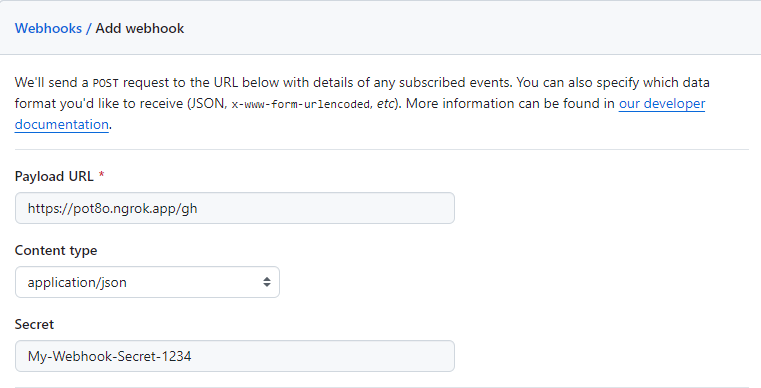
\includegraphics[width=\textwidth]{graphics/gh-webhook-1.png}
    \caption{GitHub Webhook Payload Configuration}
    \label{fig:gh-webhook-1}
\end{figure}



\FloatBarrier

\section{\cxoneflow YAML Configuration}\label{sec:gh-yaml-config}

This section is intended to show some of the GitHub-specific requirements for successful configuration.  The differences
between GitHub Enterprise and GitHub Cloud are minimal; generally the differences are related to how API and display URLs
work.

\subsection{GitHub Enterprise}

Below is a listing of a minimal GitHub Enterprise YAML configuration.  The elements to note in this
configuration:

\begin{itemize}
    \item The \texttt{base-url} is the root URL for the GitHub Enterprise instance.  This URL is also used
    when forming display links such as links to code in PR comments.
    \item The \texttt{api-url-suffix} is the path extension appended to \texttt{base-url} for API requests.
    \item Since this service definition is for a GitHub App, the \texttt{app-private-key} points to the secret
    containing the generated private key.
    \item Since the GitHub App permissions should be allowed to read repository contents, there is no need
    to provide a \texttt{clone-auth} configuration.
\end{itemize}

\begin{code}{Minimal YAML Configuration Example}{GitHub Enterprise as GitHub App}{}
secret-root-path: /run/secrets
server-base-url: https://cxoneflow.mydomain.com:8443/

gh:
    - service-name: GHE
      repo-match: .*
      feedback:
        pull-request:
          enabled: True
      connection:
        base-url: https://scm.corp.com
        api-url-suffix: api/v3
        shared-secret: scm-shared-secret
        api-auth:
          app-private-key: ghe-app-priv-key
      cxone:
        tenant: mytenant
        oauth:
          client-id: my-oauth-id
          client-secret: my-oauth-secret
        iam-endpoint: US
        api-endpoint: US
\end{code}


\subsection{GitHub Cloud}

Below is a listing of a minimal GitHub Cloud YAML configuration.  The elements to note in this
configuration:

\begin{itemize}
    \item The \texttt{base-url} is the root URL for the GitHub Cloud API.
    \item The \texttt{base-display-url} is the root URL for the GitHub Cloud UI. This URL is used
    when forming display links such as links to code in PR comments since the API URL does not
    provide interactive content.
    \item There is no \texttt{api-url-suffix} since the \texttt{base-url} is the root for API requests.
    \item Since this service definition is for a GitHub App, the \texttt{app-private-key} points to the secret
    containing the generated private key.
    \item Since the GitHub App permissions should be allowed to read repository contents, there is no need
    to provide a \texttt{clone-auth} configuration.
\end{itemize}

\begin{code}{Minimal YAML Configuration Example}{GitHub Cloud as GitHub App}{}
secret-root-path: /run/secrets
server-base-url: https://cxoneflow.mydomain.com:8443/

gh:
    - service-name: GHC
      repo-match: .*
      feedback:
        pull-request:
          enabled: True
      connection:
        base-url: https://api.github.com
        base-display-url: https://www.github.com
        shared-secret: scm-shared-secret
        api-auth:
          app-private-key: ghc-app-priv-key
      cxone:
        tenant: mytenant
        oauth:
          client-id: my-oauth-id
          client-secret: my-oauth-secret
        iam-endpoint: US
        api-endpoint: US
\end{code}
  

\section{Protected Branches}

GitHub allows a default branch to be defined for each repository.  A default branch name is defined at the organization
level and is initially inherited by each repository in the organization.  The default branch may be changed in the repository
to any branch defined in the repository. If there are no branch protection rules for the repository generating a webhook event, 
the default branch for the repository is assumed to be a protected branch.

Branch protection rules can be defined at both the organization and repository levels.  If there are any branches
defined as protected via the branch protection rules, those branches are considered protected branches.  When branch protection
rules define protected branches, the repository default branch is not considered as a protected branch unless it is also included
as a protected branch in the branch protection rules.
